\section{The Cherenkov Telescope Array}


\begin{frame}{The Cherenkov Telescope Array}
    \begin{columns}[T] % align columns
        \begin{column}{.45\textwidth}
            \vspace{10pt}
            \begin{itemize}
                \item ``Cherenkov Telescope Array''
                \item Proposed in 2005
                \item Currently in pre-production
                \item Status: First light on LST1
                \item Two arrays of multiple telescopes
                \item Three types of telescopes: LST, MST, SST
                \item Goals: Extend observable energy range, improve sensitivity, huge field of view
            \end{itemize}
        \end{column}%
        \hfill%
        \begin{column}{.53\textwidth}
            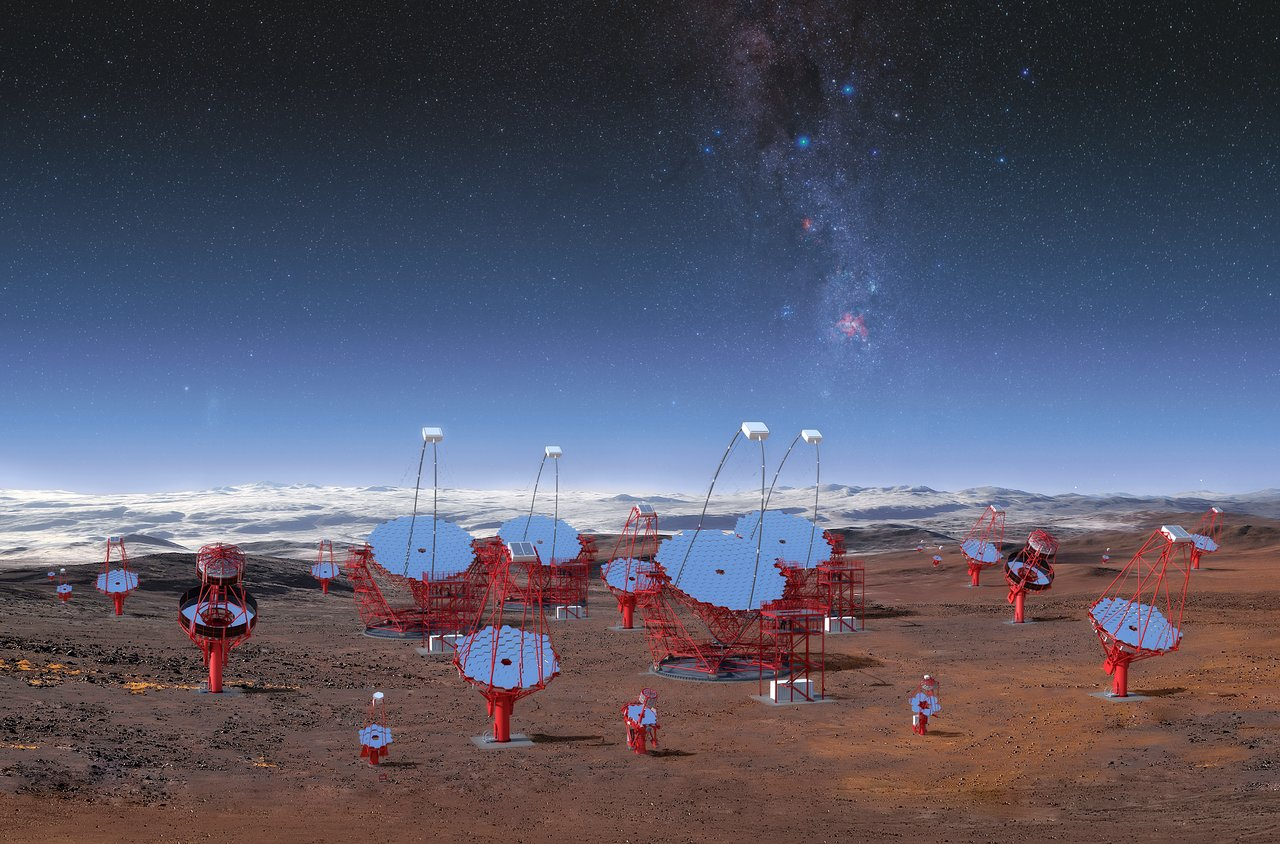
\includegraphics[width=\linewidth]{images/cta_telescopes.jpg}
            Visualization of the different telescope types.
            \footnotesize{\cite{cta_telescopes}}
        \end{column}%
    \end{columns}

\end{frame}


\begin{frame}{Planned Layout \\ \footnotesize{\cite{cta_sensitivity}}}
\centering
        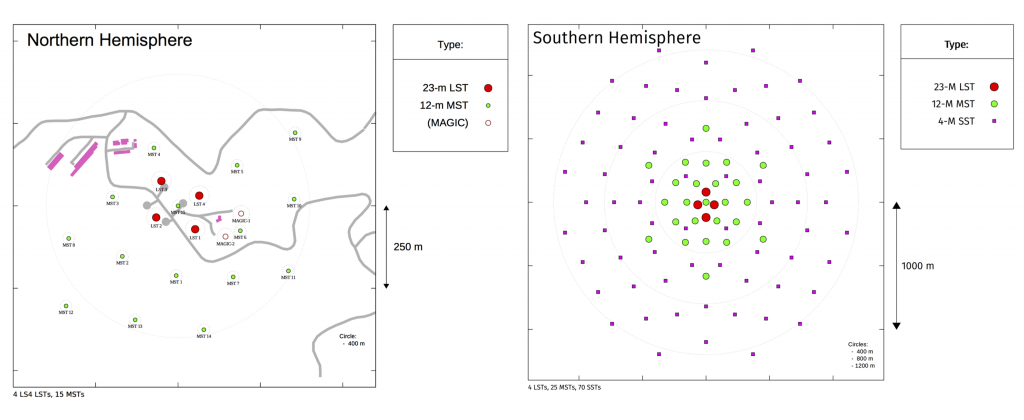
\includegraphics[width=\linewidth]{images/cta_layout.png}
\end{frame}


\begin{frame}{Expected Sensitivity \\ \footnotesize{The CTA \cite{cta_sensitivity}}}
\centering
        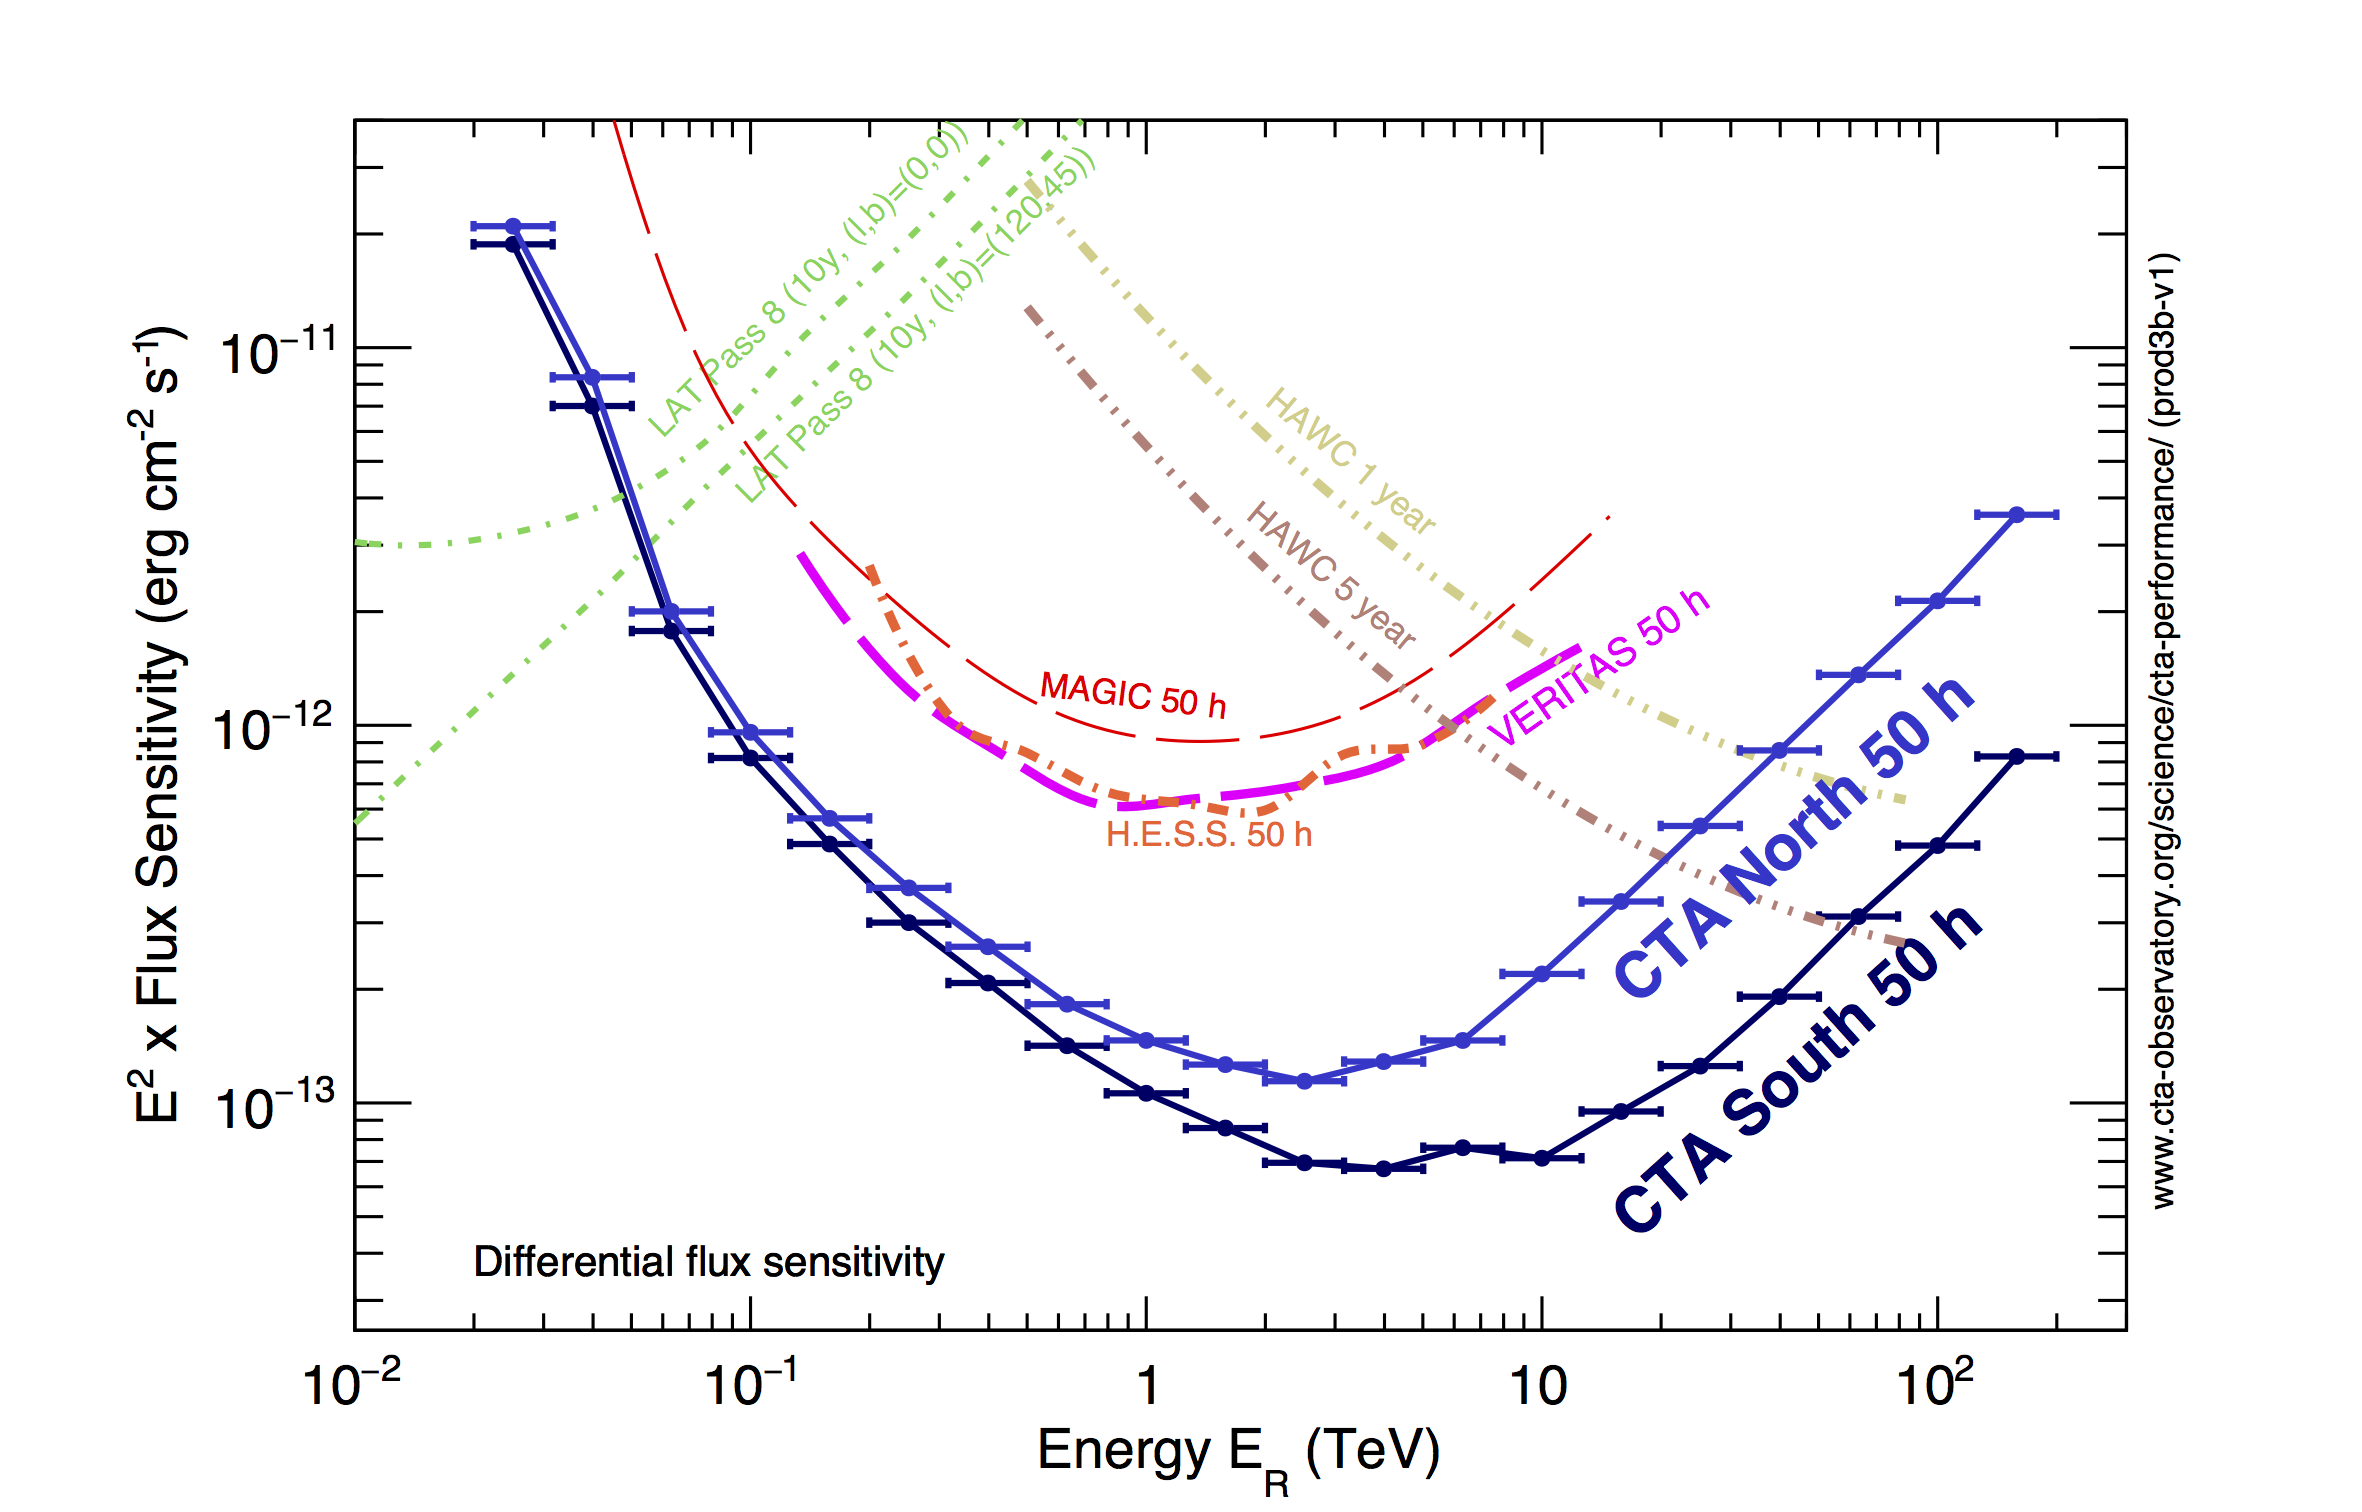
\includegraphics[width=0.7\linewidth]{images/cta_sensitivity.png}
\end{frame}

\begin{frame}{ctapipe}
    \begin{columns}[T] % align columns
        \begin{column}{.45\textwidth}
            \vspace{10pt}
            \begin{itemize}
                \item { Pipeline for lowlevel cta data}
                \item { Performs transformations, calibration, cleaning,
                        hillas parameters, 3D-reconstruction, visualization}
                \item { Still in active development}
                \item { Mainly \textbf{python} based}
                \item { https://github.com/cta-observatory/ctapipe}
            \end{itemize}
        \end{column}
        \begin{column}{.48\textwidth}
            
\includegraphics[width=\linewidth]{images/ctapipe_logo.png}
            
\includegraphics[width=\linewidth]{images/python_logo.png}
        \end{column}
    \end{columns}
\end{frame}
